\documentclass{article}
\usepackage{graphicx}
\usepackage{float}
\usepackage[acronym]{glossaries}
\usepackage{fullpage}

\loadglsentries{acronyms}
\makeglossaries

\begin{document}

\begin{tabular}{rl}
\textbf{Lab 9:} & Three Phase Induction Motor\\
\textbf{Performed:} & April 01, 2013 \\
\textbf{Partners:} & Rawley Dent \\ & Charles Pittman \\
\textbf{Instructor:} & Dr.\ Weatherford
\end{tabular}


\section*{Abstract}

In this experiment, the basic principals of operation of an induction motor
were studied.  These studies included the characteristics of a wound-rotor
induction motor analyzed at two different supply voltages.  The characteristics
such as motor speed, output torque, and line current were recorded while
varying load torque.

\section*{Results}

\begin{figure}[H]
\centering
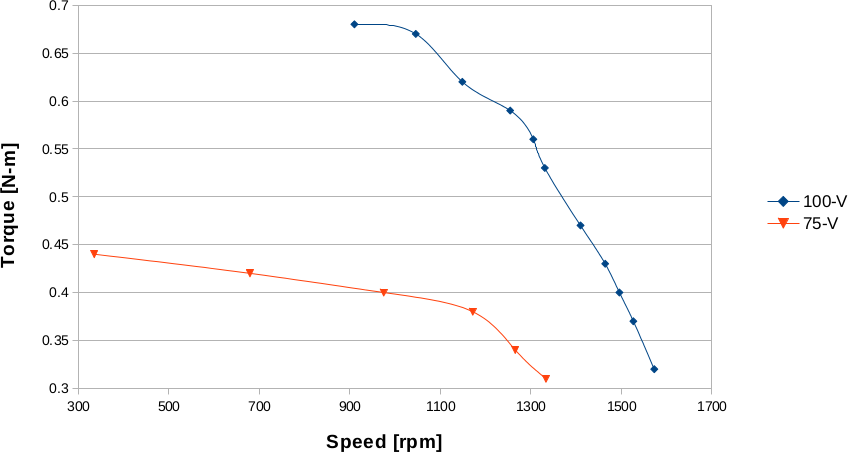
\includegraphics[width=0.7\textwidth]{img/graph}
\caption{\textbf{Comparison of Output Torque vs. Speed for Different Supply Voltages}}
\label{fig:graph}
\end{figure}

\section*{Conclusions}

In a typical torque speed curve, the plot rises sharply from the starting
torque to the breakdown (peak) torque, and then decreases linearly to the
no-load mark. This linear section, from no-load to breakdown, is the motor's
operating region.

However, the data obtained in the experiment is represented
in the figure above. The plot is not characteristic of a typical induction
motor torque-speed curve as described.  This is because of a high unknown rotor
resistance. Both supply voltages of 100-V and 75-V have the starting torques
and breakdown torques to be at the same mark. The motor with a starting voltage
of 100-V has a starting torque of 0.68-Nm and a no-load speed of 1565-rpm.  The
motor with a starting torque of 75-V had a starting torque of 0.44-Nm and a
no-load speed of 1343-rpm. Thus a wound-rotor induction motor needs to have a
higher supply voltage to be start heavy loads.

\end{document}

